\section{Analyse ISO 29002-31 - Exchange of characteristics data}

% TODO Einen definierten Großteil in den Anhang packen. Hier nur ein Beispiel und das Ergebnis erklären. 

% TODO ich habe das auskommentiert, da ich mich frage, was die Aussage am Anfang des Kapitels soll. 
%Die ISO 29002-31 ermöglicht abstrakt folgende Arten von Abfragen:
%\begin{itemize}
%\item Liefern oder validieren der bekannten und übergebenen \enquote{characteristic data} für das mittels Identifier\footnote{IRDI} angegebene Element.
%\item Liefern des Identifiers eines Elementes welches den übermittelten characteristic data (am ehesten) entspricht. 
%\end{itemize}

\subsection{XML Datencontaineranalyse ISO 29002-31}
Die Unterkapitel beschreiben die einzelnen (XML) Datencontainer aus der ISO 29002-31. Der Ausgangspunkt ist der query\_context, welcher einige Metadaten zum eigentlichen query enthält. 

\begin{figure}[htbp]
	\centering
		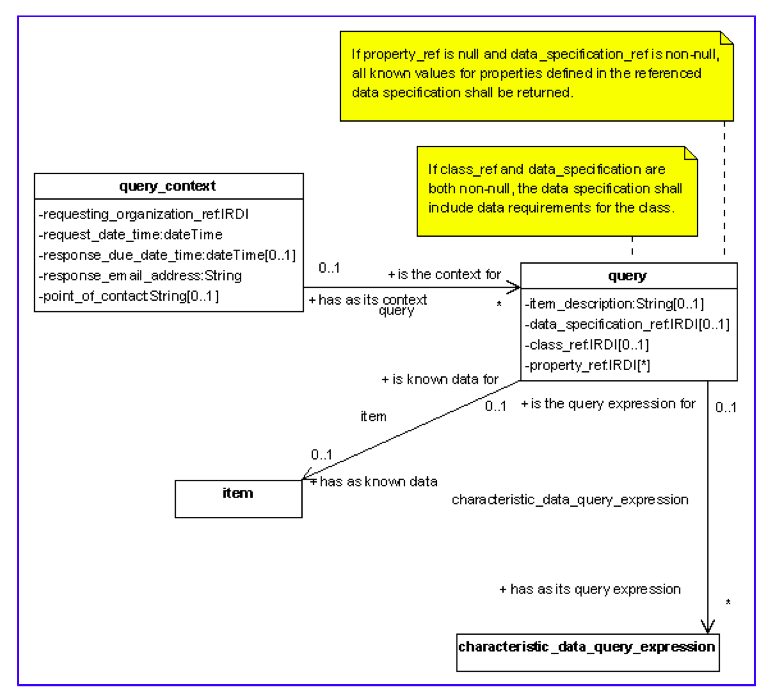
\includegraphics[width=0.99\textwidth]{images/query_main.png}
		\caption[UML-Diagramm Query Main]{UML-Diagramm Query Main\footnotemark}
	\label{fig:querymain}
\end{figure}
\footnotetext{Quelle: ISO 29002-31 Kapitel 5.2.1}

\subsubsection{query\_context}
Dies ist eine Art Container für eine Menge von Queries. Inhalt sind Informationen über den Anforderer der Daten zwecks persönlicher Kontaktaufnahme, wie z.B. die Anfragezeit, Informationen über die Organisation welche die Anfrage schickt sowie einen gewünschten Antwortzeitpunkt mit Antwort-Email Adresse. Siehe dazu Abbildung \ref{fig:querymain} und \citep[Kap. 5.2.2][]{iso29002-31}.  

Da die Vorgabe lautet, den Service auf Basis eines Web Services zu erstellen, entfällt die Benutzung des query\_context. Der Grund ist, dass der Kontext  implizit durch den Web Service respektive dem Server zur Verfügung gestellt wird. Beispielsweise wird die Anfragezeit zwar nicht explizit durch den Serviceaufrufer selbst übergeben, allerdings durch die Anfrage an den technischen Server wie z.B. Apache Tomcat Server mittels Logeintrag implizit ermittelt. Somit lassen sich diese Metadaten über Verbindungsprotokolle der Infrastruktur herausfinden.  
Siehe dazu auch \citep[Kap. 6][]{iso29002-31}, welche besagt: \\ \enquote{ISO/TS 29002 can be implemented: \\
a. with another envelope standard, such as EDI, or \\
b. by itself, using the query\_context to carry envelope information.}

\subsubsection{query}
Die Unterstützung aller Funktionalitäten des queries entspricht laut ISO 29002-31 der Conformance class 1: simple query \citep[Anhang 6][]{iso29002-31}. .
Dies ist der eigentliche Abfrage-Datensatz. Abgefragt werden kann mittels class IRDI\footnote{IRDI  - International registration data identifier}, data\_specification IRDI, eine Menge von property IRDI, Item Daten (das sind Items gefüllt mit Daten ihrer Eigenschaften die dem Klienten bereits bekannt sind) und einer item\_description. Das bedeutet, dass bereits bekannte Eigenschaften eines Teils übertragen werden können, um die Suche auf Teile mit diesen Werte-Eigenschaften einzuschränken.

Diie data\_specification IRDI verweist auf eine Spezifikation aus ISO 22745-30, die besagt welche Properties für dieses Item sinnvoll sind. Die angegebenen Property IRDIs sind dann eine Teilmenge aus den mittels data\_specification IRDI definierten erlaubten Eigenschaften. Für weitere Informationen zur ISO 22745-30 siehe Kapitel \ref{kap:identification_guide}. 

Ad hoc denkbar wären einfache Abfragen wie z.B.: \enquote{Gib mir alle Teile der Klasse xyz}. Mitgeliefert werden auch Teile von Subklassen. Weiterhin kann die Abfrage nach bestimmten Eigenschaften eingeschränkt werden. Eine weitere Möglichkeit ist es bereits bekannte Daten über ein Element zu übermitteln, mit dem Zwecke hierüber die IRDI zu erfahren oder weitere Eigenschafts-Daten zu erhalten. Siehe Beispielqueries simple queries in Kapitel \ref{kap:query_beispiele}. 

\subsubsection{characteristic\_data\_query\_expression (parametric\_query)}
Das entspricht laut ISO 29002-31 Anhang 6 der Conformance class 2: parametric query.

\begin{figure}[htbp]
	\centering
		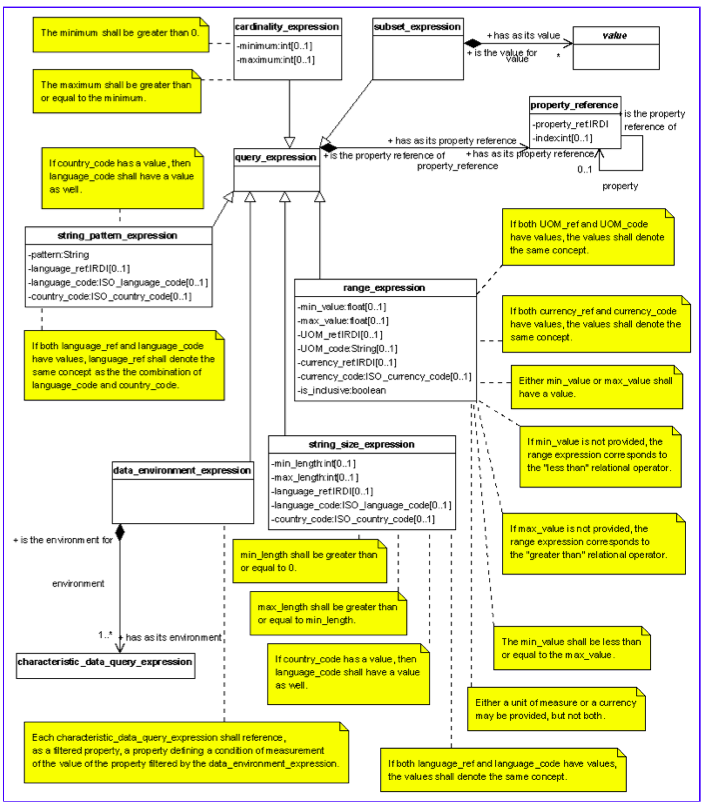
\includegraphics[width=0.99\textwidth]{images/query_expression.png}
		\caption[UML-Diagramm Query Expression]{UML-Diagramm Query Expression\footnotemark}
	\label{fig:querymain}
\end{figure}
\footnotetext{Quelle: ISO 29002-31 Kapitel 5.3.1}

Eine characteristic\_data\_query\_expression kann verschieden expressions vom Typ query\_expression beinhalten. Von jedem Typ jeweils nur maximal eine. 
Z.B.
\begin{itemize}
\item string\_size\_expression
\item string\_pattern\_expression
\item range\_expression
\item data\_environment\_expression
\item cardinality\_expression
\item subset\_expression
\end{itemize}
darüberhinaus noch folgende Attribute

\begin{itemize}
\item property\_reference - die property auf den die query\_expression bezogen ist
\end{itemize}
Solch eine Expression ermöglicht das Filtern, gleichsam ein Einschränken bestimmter Properties und Werte. 

\subsubsection{Query Beispiele}\label{kap:query_beispiele}

Nachfolgend seien einige Query-Beispielszenarien aufgestellt, die sich aus der Analyse der Standards ergeben.

Eine Schraube hat die folgenden möglichen Eigenschaften: 

\begin{description}
\item[Klassen-Identifier] 1234-abcd\# ab-cdefgh\# 1 (IRDI)
\item[Typ] M6 (Property IRDI: 1234-abcd\# ab-bbbbbb\# 1)
\item[Länge] 80mm (Property IRDI: 1234-abcd\# ab-cccccc\# 1)
\end{description}

\paragraph{Simple Query}

Ein simpler query ermöglicht folgende Abfrage: \enquote{Gib mir alle Items zu der Klasse Kreuzschraube mit dem Identifier (IRDI) 1234-abcd\#ab-cdefgh\#1}. Das Ergebnis ist ein Teil, mit allen Attributen wie oben angegeben. 

Ein anderer Query könnte lauten:  \enquote{Gib mir die Properties 1234-abcd\#ab-cccccc\#1 und 1234-abcd\#bbbbbb\# 1 des Items der Klasse 1234-abcd\#ab-cdefgh\#1}. Das Ergebnis wäre das Teil mit Typ: M6 und die Länge: 80mm.

Es könnte auch mit Hilfe von vorhandenen Daten gesucht werden, z.B.:  \enquote{Hier ist ein Item mit der Property Typ: M6 (Property IRDI: 1234-abcd\# ab-bbbbbb\# 1), gibt mir bitte dazu die Properties 1234-abcd\#ab-cccccc\#1 und 1234-abcd\# bbbbbb\#1} 

\paragraph{Parametric Query}

Hat man jetzt noch eine Schraube mit folgenden Eigenschaften:
\begin{description}
\item[Klassen-Identifier] 1234-abcd\#ab-cdefgh\#1 (IRDI)
\item[Typ] M5 (Property IRDI: 1234-abcd\#xx-bbbbbb\#1)
\item[Länge] 100mm (Property IRDI: 1234-abcd\#xx-cccccc\#1)
\end{description}


Mit Hilfe der characteristic\_data\_query\_expression sind folgende Abfragen möglich:  \enquote{Gib mir die Properties 1234-abcd\# ab-cccccc\#1 (Länge) und 1234-abcd\#bbbbbb\#1 (Typ) der Klasse Klasse 1234-abcd\#ab-cdefgh\#1 (Schraube) wo die Länge zwischen 50 und 150mm und der Typ M5 oder M6 sein soll.}

Diese ermöglicht das Filtern auf genau eine übergebene Property. Rekursive Abfragen sind auch möglich, beispielsweise wenn die gesuchte Property eine Multi-Property ist (Property: Loch als Wert zwei Properties mit Form und Durchmesser und Durchmesser soll gefiltert werden)

\subsection{Analyse ISO 22745-30 - Identification Guide}\label{kap:identification_guide}

%TODO Quelle für i-xml file aus eotd-i-xml
Ein Identification Guide beschreibt, welche Daten für ein Objekt benötigt werden, damit dies überhaupt sinnvoll für einen bestimmten Zweck eingesetzt werden kann. Der Käufer, Produktmanager oder Benutzer definiert die Anforderungen an die Daten. Ein  \enquote{Datenanforderungsstatement} wird als ein i-xml identification guide xml file erzeugt. Es wird definiert, was der Name des Artikels ist mit den charakteristischen Daten. Es wird die Frage beantwortet, welche Daten (Properties) zu einer bestimmten Klasse eines Objektes benötigt wird um den Artikeln zu kaufen oder zu sinnvoll zu verwalten. Diese Anforderungen werden von der Abfrageseite (Kundenseite) definiert, also derjenige, der Daten abfragen möchte. \(Quelle: ECCMA\_ISO\_8000\_certification.pdf\)
Ein Identification guide referenziert Konzepte eines Dictionaries um Datenanforderungen einer bestimmten Klasse zu beschreiben. (ISO 22745-30 Kapitel 5). 
Ein Datenempfänger kann eine Organisation oder eine Gruppe von Organisationen oder Firmen sein, welche ähnliche Datenanforderungen haben. Somit wird ein Identification Guide Gruppe von einer speziellen Organisation verwaltet, welche wiederum selbst Datenempfänger sein kann.  

